\section{Data exploration}
\label{sec:DataExploration}

\begin{figure}[H]
  \centering
  \includesvg[width=.6\linewidth]{Figures/hist_prec.svg}
  \caption{Histogram of precipitation.}
\end{figure}

\begin{figure}[H]
  \centering
  \includesvg[width=.6\linewidth]{Figures/hist_temp.svg}
  \caption{Histogram of temperature.}
\end{figure}

\begin{figure}[H]
  \centering
  \includesvg[width=.6\linewidth]{Figures/hist_evap.svg}
  \caption{Histogram of evaporation.}
\end{figure}

\begin{figure}[H]
  \centering
  \includesvg[width=.6\linewidth]{Figures/hist_rnof.svg}
  \caption{Histogram of surface runoff.}
\end{figure}

\begin{figure}[H]
  \centering
  \includesvg[width=.6\linewidth]{Figures/hist_streamflow.svg}
  \caption{Histogram of streamflow.}
\end{figure}

\begin{figure}[H]
  \centering
  \includesvg[width=.6\linewidth]{Figures/hist_waterlevel.svg}
  \caption{Histogram of water level.}
\end{figure}

\begin{figure}[H]
  \centering
  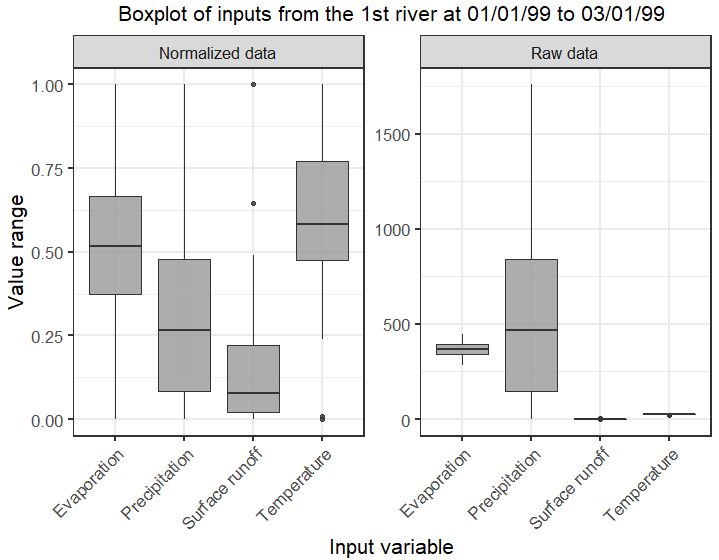
\includegraphics[width=0.8\linewidth, trim=0cm 0 0 .7cm,clip=true]{Figures/Normalização.png}
  \caption{Boxplot of inputs from normalized data (left) and raw data (right)}
  \label{fig:Normalized}
\end{figure}

\section{Parameters}
\label{sec:Parameters}
\noindent
\textbf{Support Vector Regression (SVR)}

\noindent
Kernel type: 'rbf' \\
Regularization parameter (c'): 15 to 31, step=5\\
Kernel coefficient for 'rbf' ($\gamma$)= scale/auto\\

\noindent
\textbf{Random Forest (RF)}

\noindent
The number of tree in the forest: 10, 100 or 250

\noindent
\textbf{Stacked regressor - SVR and RF}

\noindent
Combined parameters from SVR and RF.

\noindent
\textbf{Simple decision tree}

\noindent
Maximal decision tree: 5

\section{True versus predicted}
\label{sec:TrueVersusPredicted}

\begin{figure}[htbp]
  \centering
  \includesvg{Graphs/StackedComparissonFullData}
  \caption{Comparison between true and predicted values for a prediction horizon of 1 and 29 days for the whole dataset}
  \label{fig:StackedComparissonFullData}
\end{figure}